\documentclass{beamer}
\usetheme{Frankfurt}
\usecolortheme{beaver}
\setbeamertemplate{caption}{\raggedright\insertcaption\par}

\usepackage{graphicx}
\usepackage{multirow}

\def\cvs{${[}$Id: slides.tex,v 1.19 2015/12/09 16:42:43 shettyr1 Exp ${]}$}

%\beamertemplatenavigationsymbolsempty
\bibliographystyle{acm}

\newcommand{\slide}[1]{\scalebox{1.0}{\includegraphics[page=#1]{slides}}}
\begin{document}

%%-----------------------------------------------------------------------------

\title{Natural Language Description of \\Images and Videos}
\author[Rakshith Shetty]{Rakshith Shetty\\[4mm] {\small Supervisor: Professor Juha Karhunen\\ Advisor: D.\@Sc.\@ (Tech.\@) Jorma Laaksonen}}
\institute{Department of Computer Science, \\Aalto University}
\date{\today}

\frame{\titlepage} 

%%\frame{\frametitle{Table of contents}\tableofcontents} 

%%-----------------------------------------------------------------------------

\begin{frame}{Understanding Visual Media}
  \begin{itemize}
  \item<1-> Images = \{objects, attributes, relations\}\\
  \begin{figure}[h]
    \begin{columns}
    \column{.5\linewidth}
    %\hspace{-8mm}%
    \hfill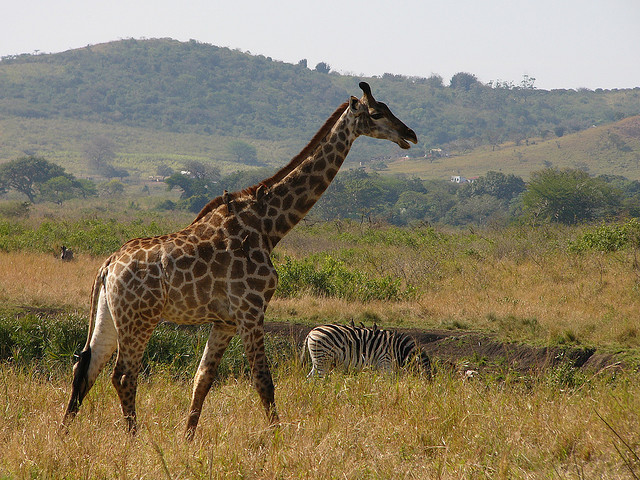
\includegraphics[width=0.6\textwidth]{images/COCO_train2014_000000544856.jpg}
    \hspace{-5mm}\column{.5\linewidth}
    \centering
    \caption{\only<5->{a giraffe walking through a patch of high dried out grass.}}
    \end{columns}
  \end{figure}
  \item<2->Videos = \{Images + temporal relations\}\\[4mm]
  \item<3->\only<3>{\Large Simple labels do not capture enough }
           \only<4>{\Large How do we summarize this information?}
           \only<5>{\Large Humans rely on natural language descriptions}
           \only<6>{\Large Can computers generate captions too?}
  \end{itemize}
\end{frame}

%%-----------------------------------------------------------------------------
\begin{frame}{Why Captioning?}
%\includegraphics[width=1\textwidth]{images/VideoCaptionModified.png}
\begin{itemize}
\item Moving beyond single label classification.
\item Better search and indexing of visual data.
\item Measure visual features and language generation.
\item Enabling better accessibility to the blind.
\item Enable computers to connect textual and visual data. 
\end{itemize}
\end{frame}
%%-----------------------------------------------------------------------------
\begin{frame}{Table of Contents}
\begin{itemize}
\item Background 
\item Baseline model
\item Enhancing visual features and language model 
\item How do we evaluate captions?
\item Results
\item What next?
\end{itemize} 

\end{frame}
%%-----------------------------------------------------------------------------

%%=============================================================================
\section{Background}
\subsection{Problem Statement and Background}
%%-----------------------------------------------------------------------------
\begin{frame}{Basic Framework}
\textbf{Given an input image or video, $V$, output a caption, $S$}
\begin{itemize}
\item<2-> $S$ is not unique
\item<3-> Learn a probabilistic model, $P(S|V)$
\item<4-> $S$, is a sequence of words $(w_0, w_1,\cdots, w_{L-1})$
\begin{equation}
\label{eq:langB1} P(S|V) = P(w_0, w_1, \cdots, w_{L-1}|V)
\end{equation}
\item<5-> Two-staged approach
    \only<5>{\begin{itemize}
        \item Visual feature extraction: $V_f = f(V)$
        \item Language modeling: $P(S|V) ~= P(S|V_f)$ 
    \end{itemize}
    }
    \only<6>{
        \begin{figure}[h]
            \centering
            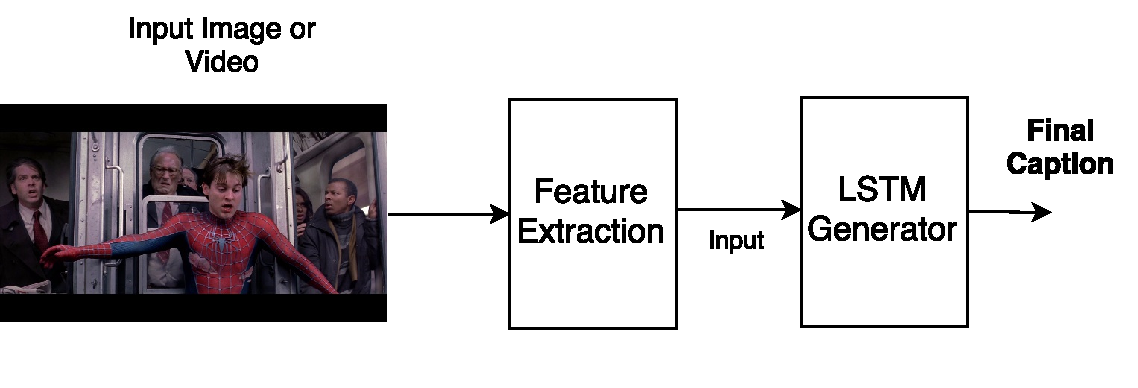
\includegraphics[width=0.8\textwidth]{images/Thesis_generalBaseline.pdf}
        \end{figure}
     }
\end{itemize} 
\end{frame}
%%-----------------------------------------------------------------------------
\begin{frame}{Techniques in Literature}
\begin{itemize}
  \item Two different approaches:
      \begin{enumerate}
        \item Retrieval-based 
        \item Generative models (Ours)
      \end{enumerate}
  \item<2-> Earliest works were retrieval based~\cite{Farhadi2010, Hodosh2013, Karpathy2014}
          {\begin{itemize}
          \item Based on common embedding on input image and textual descriptions  
      \end{itemize}}
  \item<3-> Early caption generation models were sentence template based
  \item<4-> This has been replaced with generative language models 
  \item<5-> Retrieval Vs Generative: 
      \begin{itemize}
        \item Retrieval problem: Easy to evaluate, no novelty 
        \item Generative problem: Novel captions, harder to evaluate
      \end{itemize}
\end{itemize} 
\end{frame}
%%-----------------------------------------------------------------------------
\subsection{Visual Features}
%%-----------------------------------------------------------------------------
\begin{frame}{Image Features}
\begin{itemize}
\item Deep convolutional neural networks for image classification 
    \begin{itemize}
        \item Lower layers contain convolutional filters 
        \item Followed by fully connected layers
    \end{itemize}
\item Learn hierarchical features
\item Higher layers are good out-of-the-box features  
    \begin{itemize}    
        \item Activations from fully connected layers before softmax 
    \end{itemize}
\item Widely used in recent image captioning literature~\cite{Vinyals_2015_CVPR,Fang2015} 
\end{itemize} 
\end{frame}
%%-----------------------------------------------------------------------------
\begin{frame}{Video Features}
\begin{itemize}
\item Still rely heavily on hand-crafted features
\end{itemize} 
\end{frame}
%%-----------------------------------------------------------------------------
\begin{frame}{Language Model}
\begin{itemize}
\item Traditional $n$-gram models have too short context
\item Recurrent language models address this
\item Decompose $P(S|V)$
    \begin{align*}
        \label{eq:langB2} 
        P(S|V) &= P(w_0, w_1, \cdots, w_{L-1}|V) \\
               &= p(w_0|V)p(w_1|w_0,V)p(w_2|w_1,V)\cdots p(w_{L-1}|w_{L-2},V)
    \end{align*}
\end{itemize} 
\end{frame}
%%-----------------------------------------------------------------------------
\begin{frame}{Baseline Model}
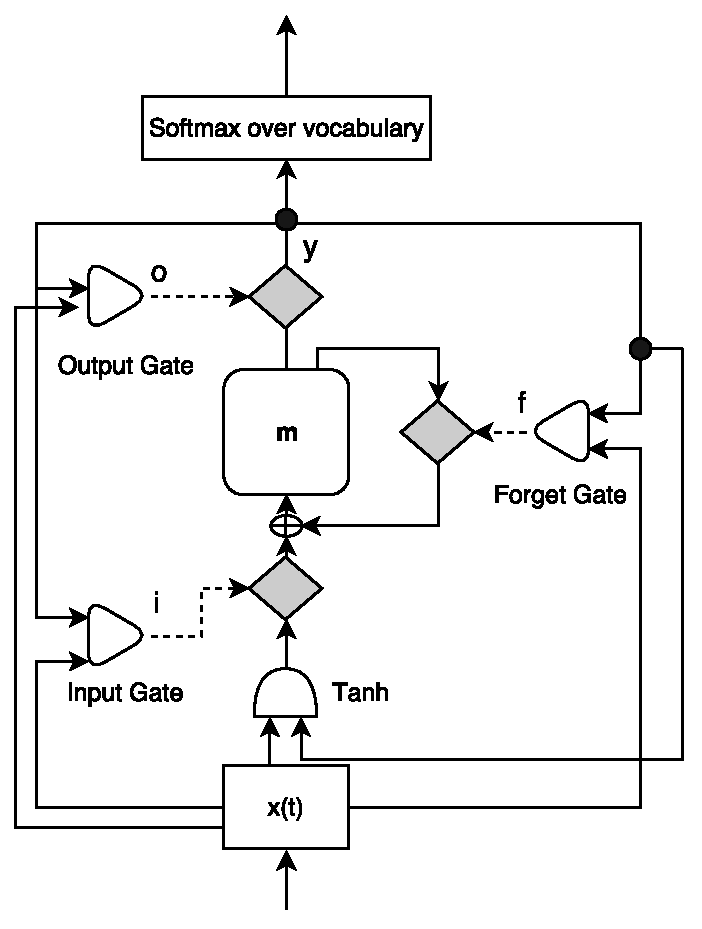
\includegraphics[width=0.3\textwidth]{images/LstmBlockDiag.pdf}
\begin{itemize}
        \item 
\end{itemize} 
\end{frame}
%%-----------------------------------------------------------------------------
%%-----------------------------------------------------------------------------
%%=============================================================================
%%=============================================================================
\section{Enhancing Language Model}
%%=============================================================================
\section{Enhancing Visual Features}
%%=============================================================================
\section{Evaluation Methods}
%%=============================================================================
\section{Results}
%%-----------------------------------------------------------------------------
\begin{frame}{Sample Validation Set Results}
    \textbf{The Good}\\[2mm]
    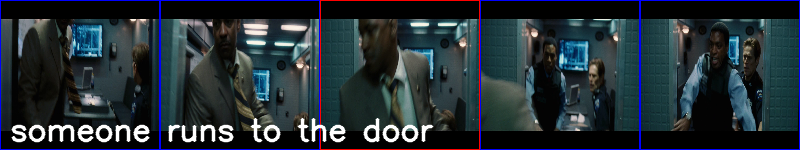
\includegraphics[width=0.5\textwidth]{images/230350439_genCap.png}\hspace*{0.01\textwidth} 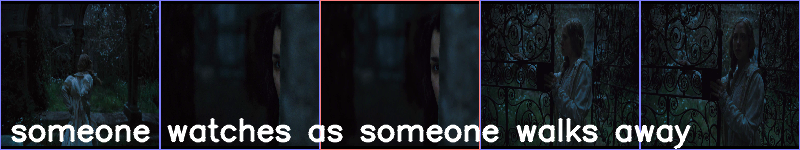
\includegraphics[width=0.5\textwidth]{images/110270280_genCapEdited.png}\\[2mm]
    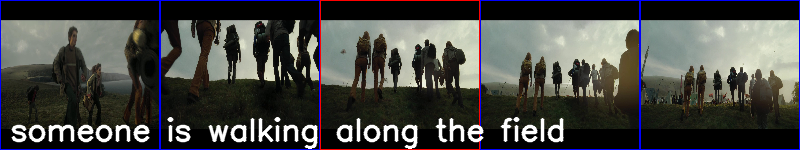
\includegraphics[width=0.5\textwidth]{images/110510033_genCap.png}\hspace*{0.01\textwidth} 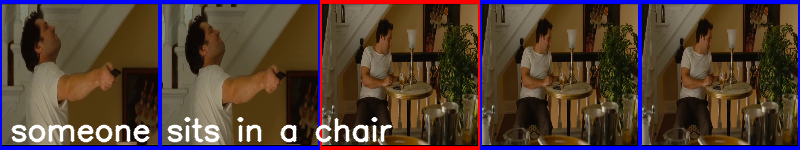
\includegraphics[width=0.5\textwidth]{images/140760125_genCap.png}\\[2mm]
    \textbf{The Bad}\\[2mm]
    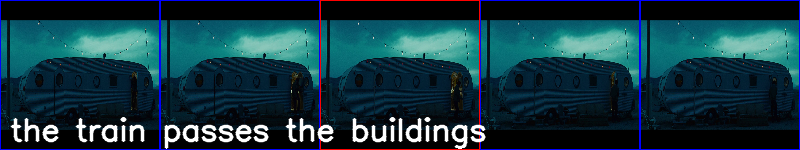
\includegraphics[width=0.5\textwidth]{images/110260059_genCap.png}\hspace*{0.01\textwidth} 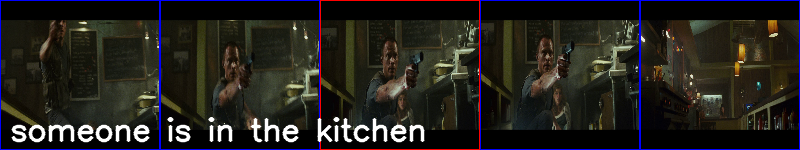
\includegraphics[width=0.5\textwidth]{images/110260532_genCap.png}\\[2mm]
    \textbf{The Ugly}\\[2mm]
    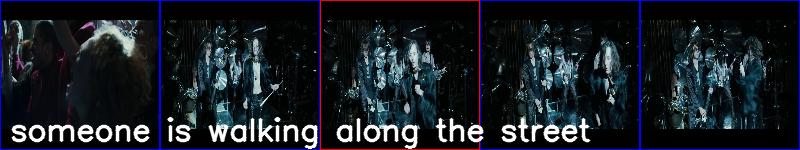
\includegraphics[width=0.5\textwidth]{images/110510496_genCap.png}\hspace*{0.01\textwidth} 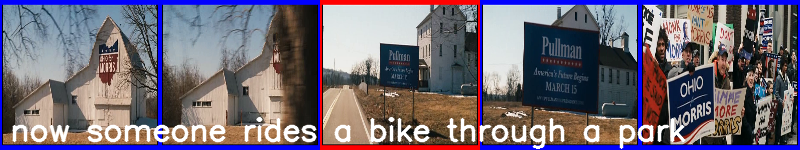
\includegraphics[width=0.5\textwidth]{images/140770020_genCap.png}\\
\end{frame}
%%=============================================================================
\section{Looking Forward}
%%-----------------------------------------------------------------------------
%%-----------------------------------------------------------------------------

\bibliography{bib_thesis_used_only}
\end{document}
